\section{Vergleich Simulation und Realität}
Um die Realitätsnähe der Simulation zu quantifizieren, wird der Ansatz über die Analyse von Aufnahmen diverser real
durchgeführter Stösse verfolgt.
Dabei ist die Geschwindigkeit, welche die Kugel zu Beginn durch den Queue erfährt, unbekannt.
Diese wird in einem ersten Schritt eruiert.
Bekannt dabei ist die Zeit sowie die Distanz, welche über die Auswahl einzelner Frames berechnet werden.
Die Zeit ergibt sich durch den Abstand zweier Frames.
Bei einem Video mit 30 FPS liegt der Fehler bei $\frac{1}{30} t [s] = 0.03 [s]$.
Die Distanz wird über zwei selektierte Pixelpositionen auf denselben Frames zur Berechnung der Zeit bestimmt.
Diese Positionen werden zu Modellkoordinaten $P_0, P_1$ übersetzt\cite{project2:pixel_to_model_coordinates},
um die Distanz in der Einheit $[mm]$ anzugeben.
Anschliessend kann über die Formel \ref{eq:simvsReal:initialVelocity} die Anfangsgeschwindigkeit berechnet
werden, wobei auch die Gleitreibung $\mu_g$ sowie die Rollreibung $\mu_r$ bekannt sein müssen\footnote{Die Herleitung
erfolgt in Kapitel \ref{anhang:herleitung:initialVelocityWithTime}.}.
\begin{align}
    v_0^2 \cdot \frac{2 \cdot (\mu_g - \mu_r)}{49 \cdot g \cdot \mu_g^2} + v_0 \cdot \frac{t \cdot (2 \cdot \mu_r + 5 \cdot \mu_g)}{7 \cdot \mu_g} - \frac{1}{2} \cdot g \cdot \mu_r \cdot t^2 - s = 0\label{eq:simvsReal:initialVelocity}
\end{align}

Es wird eine quadratische Formel gelöst, welche zwei Resultate $v^1_0, v^2_0$ liefert. Von diesen wird nur die
kleinste positive Lösung $v_0$ in Betracht gezogen.

Sobald $v_0$ bestimmt ist, kann der Geschwindigkeitsvektor $\vec{v_0}$ berechnet werden. Dies geschieht über den Einheitsvektor,
welcher über die beiden Punkte zur Bestimmung der Distanz gegeben ist:
\begin{align}
    \vec{d} &= P_1 - P_0\\
    \hat{d} &= \frac{\vec{d}}{\norm{\vec{d}}}\\
    \vec{v_0} &= v_0 \cdot \hat{d}
\end{align}

Im nächsten Schritt kann die Simulation mit der errechneten Startgeschwindigkeit des Spielballs ausgeführt werden.
Daraus resultiert eine Abfolge von Ereignissen, die in der Simulation gefunden wurden.
Diese werden mit manuell erstellten Ereignissabfolgen abgeglichen, bei welchem alle Positionen der Kugeln und Ereigniszeitpunkte
anhand der Videoaufnahmen bestimmt wurden.
Die Summe der Differenzen zwischen den erwarteten Zeiten und Positionen bilden den Gesamtfehler.

In den Informationen, welche aus den Videos extrahiert wurden, ist ein gewisser Fehler enthalten.
Zudem wird davon ausgegangen, dass bei den durchgeführten Stössen kein Spin enthalten ist, obwohl das gut möglich ist.
Damit können die entstehenden Differenzen nicht exakt verglichen werden.

\newpage
\subsection{Vergleich Stoss ohne Banden}
In diesem Abschnitt werden einige real durchgeführte und aufgezeichnete Stösse vorgestellt und die extrahierten Informationen mit
dem Resultat der Simulation verglichen.
Diese Stösse beinhalten keine Bandeninteraktionen, sondern lediglich die Interaktionen zwischen Kugeln.

\subsubsection{Stoss 1}
Im Ersten Stoss wird eine rote Kugel auf direktem Wege mit hoher Geschwindigkeit in das zentrale untere Loch gespielt.
Wegen der hohen Geschwindigkeit gleitet die weisse Kugel höchstwahrscheinlich noch bei der Kollision mit der roten Kugel.
In Abbildung \ref{fig:simulation_vs_reality_1_0008_0011} sind einige Bilder aus dem aufgezeichneten Video und ein Bild
der Simulation aufgeführt.

Für den Vergleich wurden einige Kennzahlen aus dem Video extrahiert, dies beinhaltet die Positionen der Kugeln
in Modellkoordinaten zu verschiedenen Ereignissen, sowie der Zeitpunkt (gemessen am Startzeitpunkt des Stosses) dieser Ereignisse.
In Tabelle \ref{tab:simulation_vs_reality_1_0008_0011} sind diese Kennzahlen im Vergleich und deren Differenzen aufgeführt.
Damit ist der Fehler der Simulation ersichtlich.
Der Fehler in der Position und dem Zeitpunkt des Stillstands der weissen Kugel ist vorhanden, aber gering.
In der Simulation rollt die weisse Kugel nach der Kollision noch kurz nach rechts-vorne.
Es gilt allerdings zu beachten, dass in den aus dem Video extrahierten Kennzahlen ebenfalls ein
gewisser Fehler enthalten ist, der den Vergleich schwierig macht.

\begin{figure}[h!]
    \centering
    \begin{subfigure}[t]{0.2\textwidth}
        \centering
        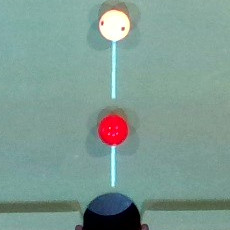
\includegraphics[width=1.0\linewidth]{../common/04_results/resources/simulation_vs_reality/simulation_vs_reality_1_0008_0011_situation_cut.jpg}
        \caption{Startsituation vor dem Stoss.}
        \label{fig:simulation_vs_reality_1_0008_0011_situation}
    \end{subfigure}
    \hfill
    \begin{subfigure}[t]{0.2\textwidth}
        \centering
        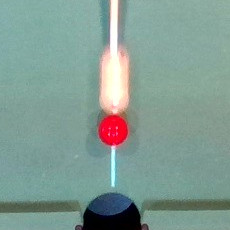
\includegraphics[width=1.0\linewidth]{../common/04_results/resources/simulation_vs_reality/simulation_vs_reality_1_0008_0011_collision_cut.jpg}
        \caption{Kollisionszeitpunkt, der \emph{motion blur} entsteht aufgrund der Geschwindigkeit der weissen Kugel.}
        \label{fig:simulation_vs_reality_1_0008_0011_collision}
    \end{subfigure}
    \hfill
    \begin{subfigure}[t]{0.2\textwidth}
        \centering
        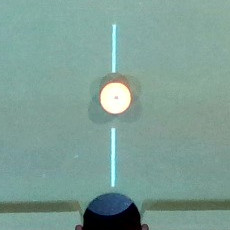
\includegraphics[width=1.0\linewidth]{../common/04_results/resources/simulation_vs_reality/simulation_vs_reality_1_0008_0011_end_cut.jpg}
        \caption{Endzustand nach dem Stoss.}
        \label{fig:simulation_vs_reality_1_0008_0011_end}
    \end{subfigure}
    \hfill
    \begin{subfigure}[t]{0.2\textwidth}
        \centering
        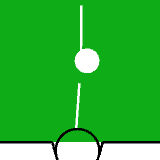
\includegraphics[width=1.0\linewidth]{../common/04_results/resources/simulation_vs_reality/simulation_vs_reality_1_0008_0011_simulation_cut.png}
        \caption{Endzustand nach dem Stoss gemäss Simulation.}
        \label{fig:simulation_vs_reality_1_0008_0011_simulation}
    \end{subfigure}
    \caption{
        Ablauf von Stoss 1: Die weisse Kugel wird mit hoher Geschwindigkeit angestossen, trifft die rote Kugel und locht diese ein.
        Die weisse Kugel steht sofort nach der Kollision still.
    }
    \label{fig:simulation_vs_reality_1_0008_0011}
\end{figure}

\begin{table}[ht]
    \rowcolors{1}{\seccolor!10}{\seccolor!10} % Rows with 10% of secondary color
    \begin{tabular}{ lrrr }
        \rowcolor{\seccolor!50}
        Kennzahl & Wert gemäss Video & Wert gemäss Simulation & Differenz \\
        Start: Position weisse Kugel & (8.38658, -159.215) & - & -\\
        Start: Position rote Kugel & (4.24078, -336.939) & - & -\\
        Kollision: Position weisse Kugel & (7.84763, -284.44) & (7.84627, -284.756) & 0.315677mm\\
        Einlochen: Zeitpunkt rote Kugel wird eingelocht & 0.133333s & 0.172932s & +0.039598s\\
        Stillstand: Position weisse Kugel & (9.53746, -284.455) & (21.7098, -285.714) & 12.237230mm\\
        Stillstand: Zeitpunkt & 0.2s & 0.530894s & +0.330895\\
    \end{tabular}
    \caption{Vergleich Video und Simulation für Stoss 1}
    \label{tab:simulation_vs_reality_1_0008_0011}
\end{table}

\subsubsection{Stoss 2}
Stoss 2 bildet dieselbe Ausgangssituation wie Stoss 1, allerdings wird die weisse Kugel mit einer tieferen Geschwindigkeit angespielt.
In Abbildung \ref{fig:simulation_vs_reality_1_0028_0032} ist der Ablauf des Stosses sowie der Endzustand der Simulation abgebildet.
Aus Tabelle \ref{tab:simulation_vs_reality_1_0028_0032} ist der Positionsfehler der weissen Kugel beim Stillstand auffallend.
Die Simulation hat die weisse Kugel nach der Kollision zu wenig weit rollen lassen.
Das kann auf die Reibungskoeffizienten, den Energieverlust bei Kugelkollision oder die eingegebene Startgeschwindigkeit zurückzuführen sein.

\begin{figure}[h!]
    \centering
    \begin{subfigure}[t]{0.2\textwidth}
        \centering
        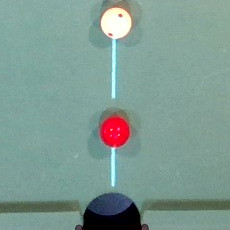
\includegraphics[width=1.0\linewidth]{../common/04_results/resources/simulation_vs_reality/simulation_vs_reality_1_0028_0032_situation_cut.jpg}
        \caption{Startsituation vor dem Stoss.}
        \label{fig:simulation_vs_reality_1_0028_0032_situation}
    \end{subfigure}
    \hfill
    \begin{subfigure}[t]{0.2\textwidth}
        \centering
        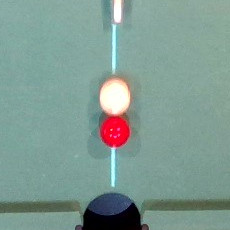
\includegraphics[width=1.0\linewidth]{../common/04_results/resources/simulation_vs_reality/simulation_vs_reality_1_0028_0032_collision_cut.jpg}
        \caption{Kollisionszeitpunkt.}
        \label{fig:simulation_vs_reality_1_0028_0032_collision}
    \end{subfigure}
    \hfill
    \begin{subfigure}[t]{0.2\textwidth}
        \centering
        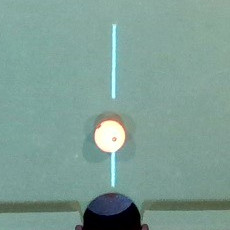
\includegraphics[width=1.0\linewidth]{../common/04_results/resources/simulation_vs_reality/simulation_vs_reality_1_0028_0032_end_cut.jpg}
        \caption{Endzustand nach dem Stoss.}
        \label{fig:simulation_vs_reality_1_0028_0032_end}
    \end{subfigure}
    \hfill
    \begin{subfigure}[t]{0.2\textwidth}
        \centering
        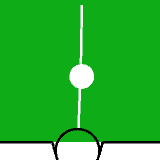
\includegraphics[width=1.0\linewidth]{../common/04_results/resources/simulation_vs_reality/simulation_vs_reality_1_0028_0032_simulation_cut.png}
        \caption{Endzustand nach dem Stoss gemäss Simulation.}
        \label{fig:simulation_vs_reality_1_0028_0032_simulation}
    \end{subfigure}
    \caption{
        Ablauf von Stoss 2: Die weisse Kugel wird mit tiefer Geschwindigkeit angestossen, trifft die rote Kugel und locht diese ein.
        Die weisse Kugel rollt nach der Kollision noch kurz nach vorne.
    }
    \label{fig:simulation_vs_reality_1_0028_0032}
\end{figure}

\begin{table}[ht]
    \rowcolors{1}{\seccolor!10}{\seccolor!10} % Rows with 10% of secondary color
    \begin{tabular}{ lrrr }
        \rowcolor{\seccolor!50}
        Kennzahl & Wert gemäss Video & Wert gemäss Simulation & Differenz \\
        Start: Position weisse Kugel & (9.99188, -157.766) & - & -\\
        Start: Position rote Kugel & (5.8054, -342.29) & - & -\\
        Kollision: Position weisse Kugel & (7.72594, -289.771) & (7.72172, -290.017) & 0.245703mm\\
        Einlochen: Zeitpunkt rote Kugel wird eingelocht & 0.7s & 0.687573s & -0.012427s\\
        Stillstand: Position weisse Kugel & (-2.68527, -350.685) & (9.62618, -321.478) & 31.695890mm\\
        Stillstand: Zeitpunkt & 1.3s & 0.972639s & -0.327361s\\
    \end{tabular}
    \caption{Vergleich Video und Simulation für Stoss 2}
    \label{tab:simulation_vs_reality_1_0028_0032}
\end{table}

\subsubsection{Stoss 3}
In dieser Situation wird eine rote Kugel in einem Winkel von der weissen Kugel mit einer kleinen Geschwindigkeit angespielt.
Die beiden Kugeln rollen nach der Kollision eine kurze Zeit weiter und kommen dann zum Stillstand.
Der Ablauf ist in Abbildung \ref{fig:video_12_0205_0208} und der Vergleich in Tabelle \ref{tab:video_12_0205_0208} dargestellt.
Zusätzlich zu den Positionen und Zeiten der Ereignisse sind zusätzlich die Richtungen, in welche die Kugeln nach der Kollision
rollen, enthalten.
Der Positionsfehler beträgt beim Stillstand ca. 2cm und die Richtung unterscheidet sich bei der roten Kugel um $7^{\circ}$.

\begin{figure}[h!]
    \centering
    \begin{subfigure}[t]{0.2\textwidth}
        \centering
        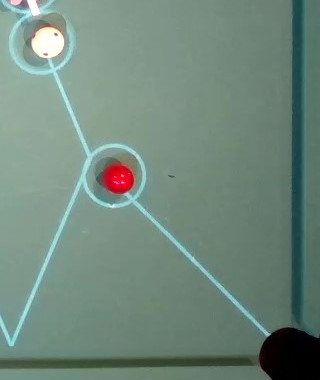
\includegraphics[width=1.0\linewidth]{../common/04_results/resources/simulation_vs_reality/video_12_0205_0208_situation_cut.jpg}
        \caption{Startsituation vor dem Stoss.}
        \label{fig:video_12_0205_0208_situation}
    \end{subfigure}
    \hfill
    \begin{subfigure}[t]{0.2\textwidth}
        \centering
        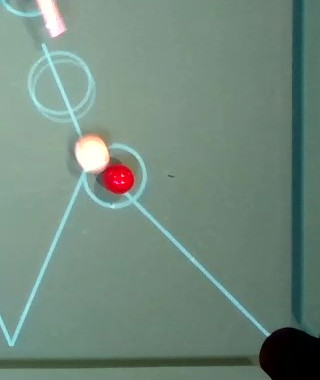
\includegraphics[width=1.0\linewidth]{../common/04_results/resources/simulation_vs_reality/video_12_0205_0208_collision_cut.jpg}
        \caption{Kollisionszeitpunkt.}
        \label{fig:video_12_0205_0208_collision}
    \end{subfigure}
    \hfill
    \begin{subfigure}[t]{0.2\textwidth}
        \centering
        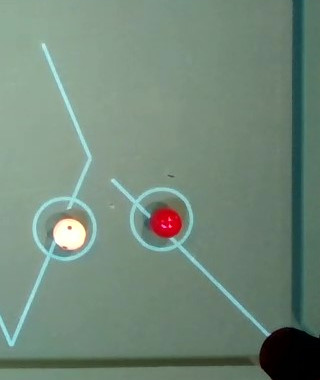
\includegraphics[width=1.0\linewidth]{../common/04_results/resources/simulation_vs_reality/video_12_0205_0208_end_cut.jpg}
        \caption{Endzustand nach dem Stoss.}
        \label{fig:video_12_0205_0208_end}
    \end{subfigure}
    \hfill
    \begin{subfigure}[t]{0.2\textwidth}
        \centering
        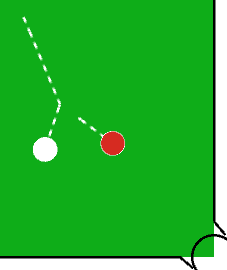
\includegraphics[width=1.0\linewidth]{../common/04_results/resources/simulation_vs_reality/video_12_0205_0208_simulation_cut.png}
        \caption{Endzustand nach dem Stoss gemäss Simulation.}
        \label{fig:video_12_0205_0208_simulation}
    \end{subfigure}
    \caption{
        Ablauf von Stoss 3: Die weisse Kugel wird mit tiefer Geschwindigkeit angestossen und trifft die rote Kugel.
        Beide Kugeln rollen nach der Kollision weiter und bleiben nach kurzer Zeit stehen.
    }
    \label{fig:video_12_0205_0208}
\end{figure}

\begin{table}[ht]
    \rowcolors{1}{\seccolor!10}{\seccolor!10} % Rows with 10% of secondary color
    \begin{tabular}{ lrrr }
        \rowcolor{\seccolor!50}
        Kennzahl & Wert gemäss Video & Wert gemäss Simulation & Differenz \\
        Start: Position weisse Kugel & (504.88, 77.68) & - & -\\
        Start: Position rote Kugel & (630.137, -152.789) & - & -\\
        Kollision: Position weisse Kugel & (585.423, -114.962) & (588.18, -121.556) & 7.146715mm\\
        Rollen nach Kollision: Richtung weisse Kugel & (-0.288612, -0.957446) & (-0.309209, -0.950994) & 1.236697$^{\circ}$ \\
        Rollen nach Kollision: Richtung rote Kugel & (0.715309, -0.698809) & (0.802148, -0.597126) & 7.667131$^{\circ}$ \\
        Stillstand: Position weisse Kugel & (545.906, -246.056) & (554.434, -225.344) & 22.398825mm\\
        Stillstand: Zeitpunkt weisse Kugel & 2.233333s & 1.909805s & -0.323528s\\
        Stillstand: Position rote Kugel & (709.469, -230.291) & (709.088, -211.561) & 18.734226mm\\
        Stillstand: Zeitpunkt rote Kugel & 1.933333s & 1.840109s & -0.093224s\\
    \end{tabular}
    \caption{Vergleich Video und Simulation für Stoss 3}
    \label{tab:video_12_0205_0208}
\end{table}

\newpage
\subsubsection{Stoss 4}
Mit Stoss 4 wird die rote Kugel in gerader Linie von der weissen Kugel mit mittlerer Geschwindigkeit eingelocht,
siehe Abbildung \ref{fig:video_13_0030_0034}.
Aus Tabelle \ref{tab:video_13_0030_0034} sind kleine zeitliche Differenzen ersichtlich und
ein Positionsfehler beim Stillstand der weissen Kugel von 2,6cm.

\begin{figure}[h!]
    \centering
    \begin{subfigure}[t]{0.2\textwidth}
        \centering
        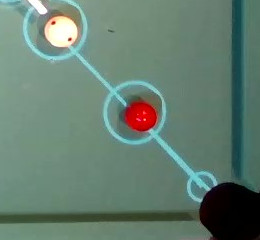
\includegraphics[width=1.0\linewidth]{../common/04_results/resources/simulation_vs_reality/video_13_0030_0034_situation_cut.jpg}
        \caption{Startsituation vor dem Stoss.}
        \label{fig:video_13_0030_0034_situation}
    \end{subfigure}
    \hfill
    \begin{subfigure}[t]{0.2\textwidth}
        \centering
        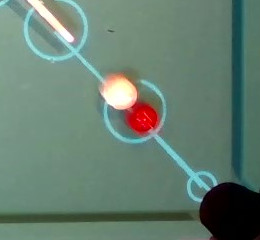
\includegraphics[width=1.0\linewidth]{../common/04_results/resources/simulation_vs_reality/video_13_0030_0034_collision_cut.jpg}
        \caption{Kollisionszeitpunkt.}
        \label{fig:video_13_0030_0034_collision}
    \end{subfigure}
    \hfill
    \begin{subfigure}[t]{0.2\textwidth}
        \centering
        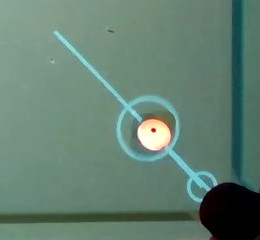
\includegraphics[width=1.0\linewidth]{../common/04_results/resources/simulation_vs_reality/video_13_0030_0034_end_cut.jpg}
        \caption{Endzustand nach dem Stoss.}
        \label{fig:video_13_0030_0034_end}
    \end{subfigure}
    \hfill
    \begin{subfigure}[t]{0.2\textwidth}
        \centering
        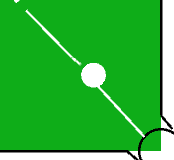
\includegraphics[width=1.0\linewidth]{../common/04_results/resources/simulation_vs_reality/video_13_0030_0034_simulation_cut.png}
        \caption{Endzustand nach dem Stoss gemäss Simulation.}
        \label{fig:video_13_0030_0034_simulation}
    \end{subfigure}
    \caption{
        Ablauf von Stoss 4: Die weisse Kugel wird mit mittlerer Geschwindigkeit angestossen, trifft die rote Kugel und locht diese ein.
        Die weisse Kugel rollt nach der Kollision noch kurz nach vorne.
    }
    \label{fig:video_13_0030_0034}
\end{figure}

\begin{table}[ht]
    \rowcolors{1}{\seccolor!10}{\seccolor!10} % Rows with 10% of secondary color
    \begin{tabular}{ lrrr }
        \rowcolor{\seccolor!50}
        Kennzahl & Wert gemäss Video & Wert gemäss Simulation & Differenz \\
        Start: Position weisse Kugel & (631.828, -149.426) & - & -\\
        Start: Position rote Kugel & (771.566, -295.777) & - & -\\
        Kollision: Position weisse Kugel & (735.251, -256.098) & (736.286, -257.165) & 1.486228mm\\
        Einlochen: Zeitpunkt rote Kugel wird eingelocht & 0.8s & 0.765598s & -0.034402s\\
        Stillstand: Position weisse Kugel & (792.353, -323.378) & (786.198, -297.818) & 26.290272mm\\
        Stillstand: Zeitpunkt & 1.2s & 1.196382s & -0.003618s\\
    \end{tabular}
    \caption{Vergleich Video und Simulation für Stoss 4}
    \label{tab:video_13_0030_0034}
\end{table}

Damit wurden anhand einiger Stösse, welche keine Bandeninteraktion enthalten,
der Vergleich zwischen Simulation und Realität gezogen und quantitativ ausgewertet.
Die Auswertung ist nicht fehlerfrei, gibt allerdings einen Rahmen, in dem sich die Genauigkeit der Simulation in diesen
Situationen bewegt.

\newpage
\subsection{Vergleich Bandenstoss}\label{kap:vergleich_simulation_realitaet:vergleich_bandenstoss}
Dieses Kapitel widmet sich dem Abgleich des erwarteten Verhaltens bei einer Bandenkollision wie in
Abschnitt \ref{kandidatensuche:bandenkollisionstheorie} beschrieben und dem effektiven Verhalten des verwendeten Tisches.
Es wird in zwei Subkapitel gegliedert, wobei sich das Erste mit der Beschreibung der Realität befasst, das Zweite hingegen
mit der Diskussion der Resultate.

\subsubsection{Bandenkollisionsrealität}
Es folgt die Beschreibung eines experimentellen Vorgehens, um zu prüfen, ob die Banden des verwendeten Billardtisches den
bekannten theoretischen und praktischen Vorgaben entsprechen. Dafür wurden zwei Videos aufgenommen und analysiert,
die einen schwächeren und einen starken Stoss zeigen.
Nach der beschriebenen Theorie müsste der Ausfallswinkel in etwa dem Einfallswinkel entsprechen.
Um einen Anhaltspunkt zu gewinnen, wurde ein Stoss
über eine Bande gesucht. Dadurch werden Linien auf den Tisch projiziert, die die Ausführung des Experiments vereinfachen.
Die angestossene Kugel müsste den visualisierten Linien folgen, sollte die Theorie auf den verwendeten Billardtisch
anwendbar sein.

Beim nachfolgend präsentierten schwachen Stoss in Abbildung \ref{fig:kugelverlauf_nach_bandenkollision_mit_schwachem_stoss_pool} wird erwartet, dass der Ausfallswinkel gemäss dem Prinzip 6.7 aus
Abschnitt \ref{kandidatensuche:bandenkollisionstheorie} grösser ausfällt. Dem ist effektiv so, jedoch ist
der Ausfallswinkel viel zu gross und kommt nicht durch den beschriebenen Topspin zustande, da die Kugel zu Beginn
eigentlich durchaus dem theoretischen Ausfallsweg folgen sollte. In Abbildung \ref{fig:rebound_angle_no_spin_slow_shot} sind
einzelne Frames des Stosses ersichtlich. Bis zum Bandenaufprall folg die weisse Kugel dem erwarteten Pfad. Bereits nach
dem Bandenaufprall in $f$ kann eine leichte seitliche Verschiebung der Kugel erkannt werden, welche den weiteren Verlauf
stark beeinflusst.

\begin{figure}[h!]
    \centering
    \begin{subfigure}[b]{0.2\textwidth}
        \centering
        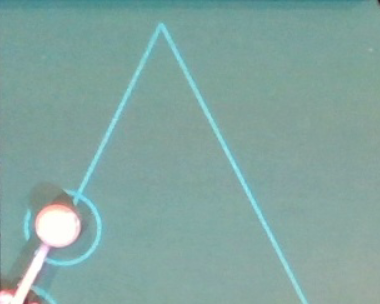
\includegraphics[width=1.0\linewidth]{../common/04_results/resources/simulation/rebound_angle_slow_pool/00_rail_rebound_angle_slow_pool_01.png}
        \caption{Ausfallswinkel bei schwachem Stoss in Pool - 1}
        \label{fig:rebound_angle_slow_pool_1}
    \end{subfigure}
    \hfill
    \begin{subfigure}[b]{0.2\textwidth}
        \centering
        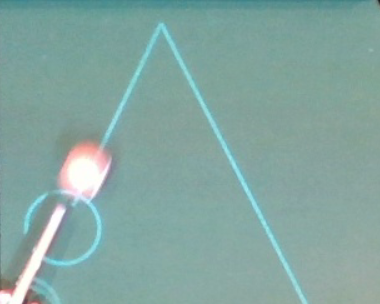
\includegraphics[width=1.0\linewidth]{../common/04_results/resources/simulation/rebound_angle_slow_pool/00_rail_rebound_angle_slow_pool_02.png}
        \caption{Ausfallswinkel bei schwachem Stoss in Pool - 2}
        \label{fig:rebound_angle_slow_pool_2}
    \end{subfigure}
    \hfill
    \begin{subfigure}[b]{0.2\textwidth}
        \centering
        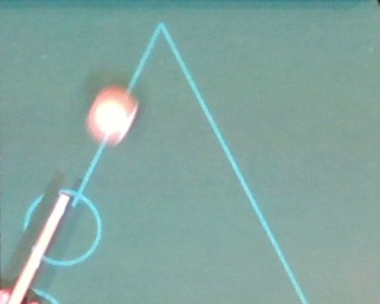
\includegraphics[width=1.0\linewidth]{../common/04_results/resources/simulation/rebound_angle_slow_pool/00_rail_rebound_angle_slow_pool_03.png}
        \caption{Ausfallswinkel bei schwachem Stoss in Pool - 3}
        \label{fig:rebound_angle_slow_pool_3}
    \end{subfigure}
    \hfill
    \begin{subfigure}[b]{0.2\textwidth}
        \centering
        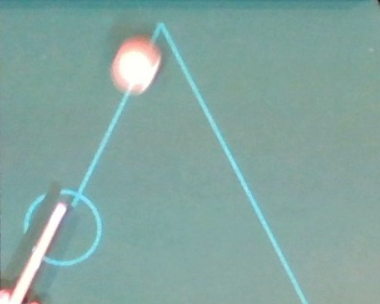
\includegraphics[width=1.0\linewidth]{../common/04_results/resources/simulation/rebound_angle_slow_pool/00_rail_rebound_angle_slow_pool_04.png}
        \caption{Ausfallswinkel bei schwachem Stoss in Pool - 4}
        \label{fig:rebound_angle_slow_pool_4}
    \end{subfigure}
    \hfill
    \begin{subfigure}[b]{0.2\textwidth}
        \centering
        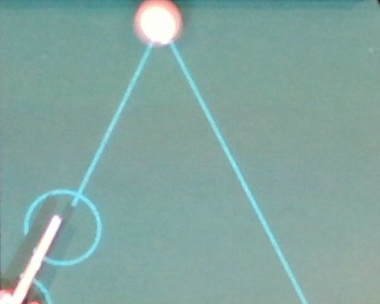
\includegraphics[width=1.0\linewidth]{../common/04_results/resources/simulation/rebound_angle_slow_pool/00_rail_rebound_angle_slow_pool_05.png}
        \caption{Ausfallswinkel bei schwachem Stoss in Pool - 5}
        \label{fig:rebound_angle_slow_pool_5}
    \end{subfigure}
    \hfill
    \begin{subfigure}[b]{0.2\textwidth}
        \centering
        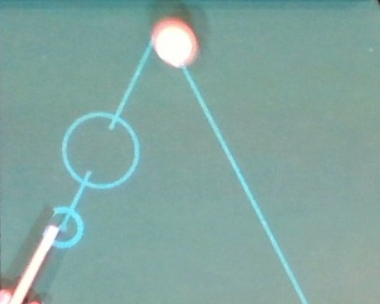
\includegraphics[width=1.0\linewidth]{../common/04_results/resources/simulation/rebound_angle_slow_pool/00_rail_rebound_angle_slow_pool_06.png}
        \caption{Ausfallswinkel bei schwachem Stoss in Pool - 6}
        \label{fig:rebound_angle_slow_pool_6}
    \end{subfigure}
    \hfill
    \begin{subfigure}[b]{0.2\textwidth}
        \centering
        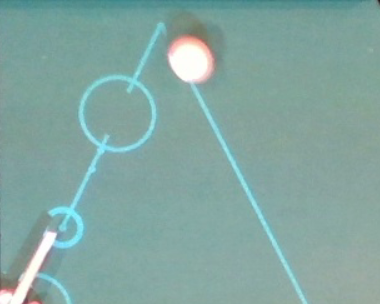
\includegraphics[width=1.0\linewidth]{../common/04_results/resources/simulation/rebound_angle_slow_pool/00_rail_rebound_angle_slow_pool_07.png}
        \caption{Ausfallswinkel bei schwachem Stoss in Pool - 7}
        \label{fig:rebound_angle_slow_pool_7}
    \end{subfigure}
    \hfill
    \begin{subfigure}[b]{0.2\textwidth}
        \centering
        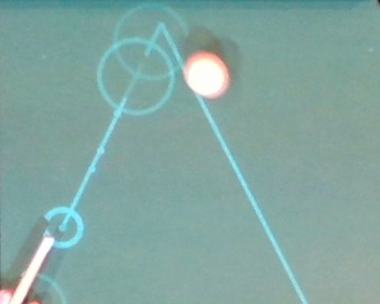
\includegraphics[width=1.0\linewidth]{../common/04_results/resources/simulation/rebound_angle_slow_pool/00_rail_rebound_angle_slow_pool_08.png}
        \caption{Ausfallswinkel bei schwachem Stoss in Pool - 8}
        \label{fig:rebound_angle_slow_pool_8}
    \end{subfigure}
    \hfill
    \begin{subfigure}[b]{0.2\textwidth}
        \centering
        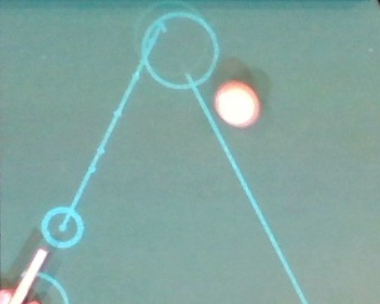
\includegraphics[width=1.0\linewidth]{../common/04_results/resources/simulation/rebound_angle_slow_pool/00_rail_rebound_angle_slow_pool_09.png}
        \caption{Ausfallswinkel bei schwachem Stoss in Pool - 9}
        \label{fig:rebound_angle_slow_pool_9}
    \end{subfigure}
    \hfill
    \begin{subfigure}[b]{0.2\textwidth}
        \centering
        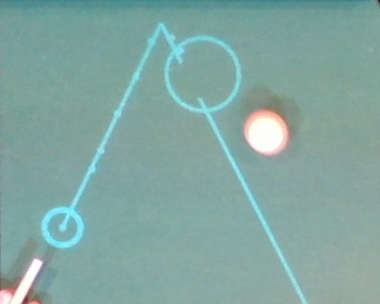
\includegraphics[width=1.0\linewidth]{../common/04_results/resources/simulation/rebound_angle_slow_pool/00_rail_rebound_angle_slow_pool_10.png}
        \caption{Ausfallswinkel bei schwachem Stoss in Pool - 10}
        \label{fig:rebound_angle_slow_pool_10}
    \end{subfigure}
    \hfill
    \begin{subfigure}[b]{0.2\textwidth}
        \centering
        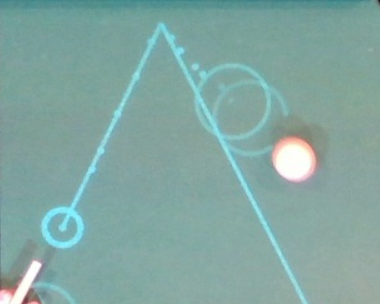
\includegraphics[width=1.0\linewidth]{../common/04_results/resources/simulation/rebound_angle_slow_pool/00_rail_rebound_angle_slow_pool_11.png}
        \caption{Ausfallswinkel bei schwachem Stoss in Pool - 11}
        \label{fig:rebound_angle_slow_pool_11}
    \end{subfigure}
    \hfill
    \begin{subfigure}[b]{0.2\textwidth}
        \centering
        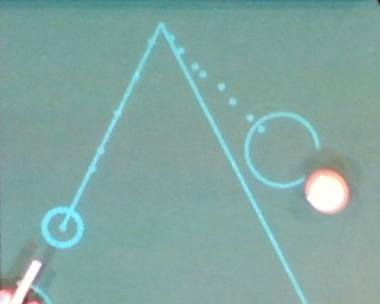
\includegraphics[width=1.0\linewidth]{../common/04_results/resources/simulation/rebound_angle_slow_pool/00_rail_rebound_angle_slow_pool_12.png}
        \caption{Ausfallswinkel bei schwachem Stoss in Pool - 12}
        \label{fig:rebound_angle_slow_pool_12}
    \end{subfigure}
    \caption{Kugelverlauf nach Bandenkollision mit schwachem Stoss - Pool}
    \label{fig:kugelverlauf_nach_bandenkollision_mit_schwachem_stoss_pool}
\end{figure}

Der starke Stoss wird in Abbildung \ref{fig:kugelverlauf_nach_bandenkollision_mit_starkem_stoss_pool} thematisiert.
Erwartet wird nach dem Prinzip 6.6 aus Kapitel \ref{kandidatensuche:bandenkollisionstheorie} ein kleinerer Ausfallswinkel als der Eingezeichnete.
Effektiv resultiert aber auch in diesem Fall wie im vorherig beschriebenen Fall ein grösserer Ausfallswinkel.
Nach dem Bandenaufprall in $f$ kann ebenso wieder eine leichte Versetzung der Kugel ausgemacht werden, die einen
grossen Einfluss hat.

\begin{figure}[h!]
    \centering
    \begin{subfigure}[b]{0.2\textwidth}
        \centering
        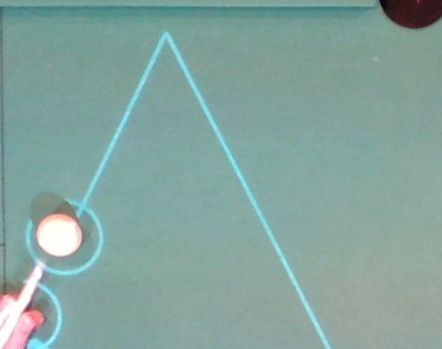
\includegraphics[width=1.0\linewidth]{../common/04_results/resources/simulation/rebound_angle_fast_pool/00_rail_rebound_angle_fast_pool_01.png}
        \caption{Ausfallswinkel bei starkem Stoss in Pool - 1}
        \label{fig:rebound_angle_fast_pool_1}
    \end{subfigure}
    \hfill
    \begin{subfigure}[b]{0.2\textwidth}
        \centering
        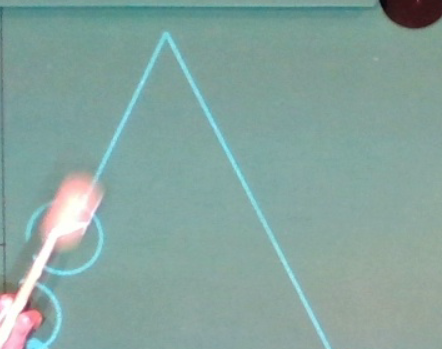
\includegraphics[width=1.0\linewidth]{../common/04_results/resources/simulation/rebound_angle_fast_pool/00_rail_rebound_angle_fast_pool_02.png}
        \caption{Ausfallswinkel bei starkem Stoss in Pool - 2}
        \label{fig:rebound_angle_fast_pool_2}
    \end{subfigure}
    \hfill
    \begin{subfigure}[b]{0.2\textwidth}
        \centering
        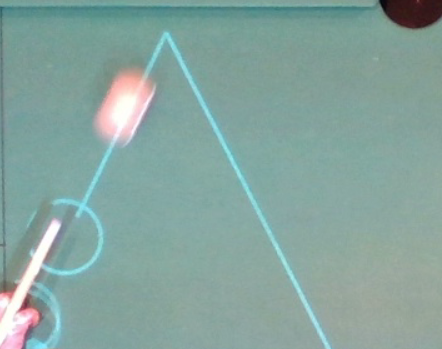
\includegraphics[width=1.0\linewidth]{../common/04_results/resources/simulation/rebound_angle_fast_pool/00_rail_rebound_angle_fast_pool_03.png}
        \caption{Ausfallswinkel bei starkem Stoss in Pool - 3}
        \label{fig:rebound_angle_fast_pool_3}
    \end{subfigure}
    \hfill
    \begin{subfigure}[b]{0.2\textwidth}
        \centering
        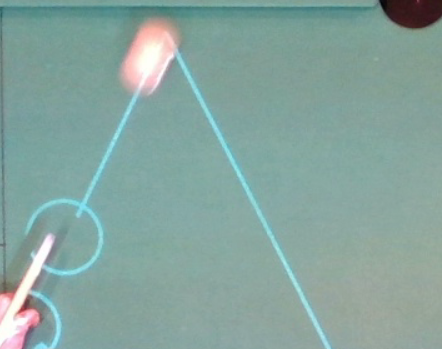
\includegraphics[width=1.0\linewidth]{../common/04_results/resources/simulation/rebound_angle_fast_pool/00_rail_rebound_angle_fast_pool_04.png}
        \caption{Ausfallswinkel bei starkem Stoss in Pool - 4}
        \label{fig:rebound_angle_fast_pool_4}
    \end{subfigure}
    \hfill
    \begin{subfigure}[b]{0.2\textwidth}
        \centering
        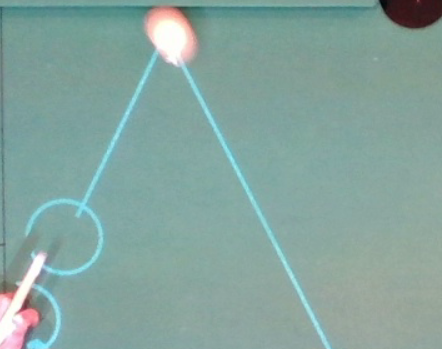
\includegraphics[width=1.0\linewidth]{../common/04_results/resources/simulation/rebound_angle_fast_pool/00_rail_rebound_angle_fast_pool_05.png}
        \caption{Ausfallswinkel bei starkem Stoss in Pool - 5}
        \label{fig:rebound_angle_fast_pool_5}
    \end{subfigure}
    \hfill
    \begin{subfigure}[b]{0.2\textwidth}
        \centering
        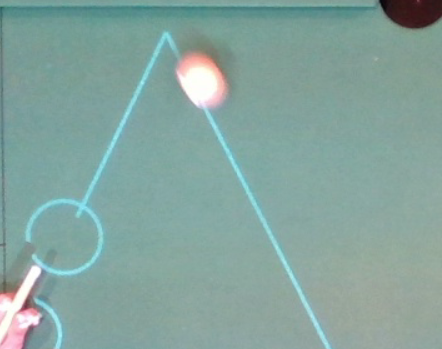
\includegraphics[width=1.0\linewidth]{../common/04_results/resources/simulation/rebound_angle_fast_pool/00_rail_rebound_angle_fast_pool_06.png}
        \caption{Ausfallswinkel bei starkem Stoss in Pool - 6}
        \label{fig:rebound_angle_fast_pool_6}
    \end{subfigure}
    \hfill
    \begin{subfigure}[b]{0.2\textwidth}
        \centering
        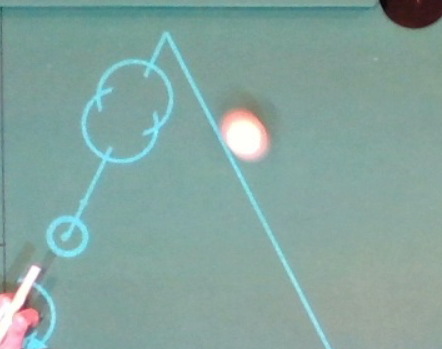
\includegraphics[width=1.0\linewidth]{../common/04_results/resources/simulation/rebound_angle_fast_pool/00_rail_rebound_angle_fast_pool_07.png}
        \caption{Ausfallswinkel bei starkem Stoss in Pool - 7}
        \label{fig:rebound_angle_fast_pool_7}
    \end{subfigure}
    \hfill
    \begin{subfigure}[b]{0.2\textwidth}
        \centering
        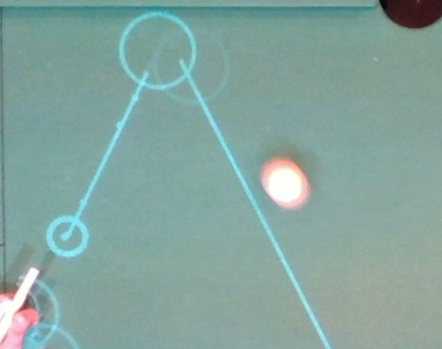
\includegraphics[width=1.0\linewidth]{../common/04_results/resources/simulation/rebound_angle_fast_pool/00_rail_rebound_angle_fast_pool_08.png}
        \caption{Ausfallswinkel bei starkem Stoss in Pool - 8}
        \label{fig:rebound_angle_fast_pool_8}
    \end{subfigure}
    \hfill
    \begin{subfigure}[b]{0.2\textwidth}
        \centering
        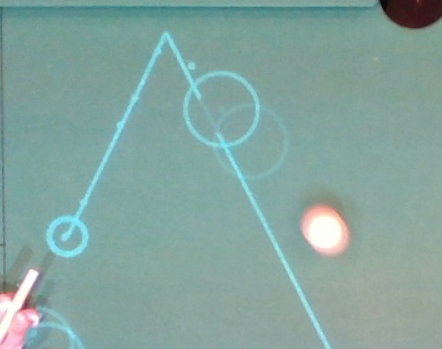
\includegraphics[width=1.0\linewidth]{../common/04_results/resources/simulation/rebound_angle_fast_pool/00_rail_rebound_angle_fast_pool_09.png}
        \caption{Ausfallswinkel bei starkem Stoss in Pool - 9}
        \label{fig:rebound_angle_fast_pool_9}
    \end{subfigure}
    \hfill
    \begin{subfigure}[b]{0.2\textwidth}
        \centering
        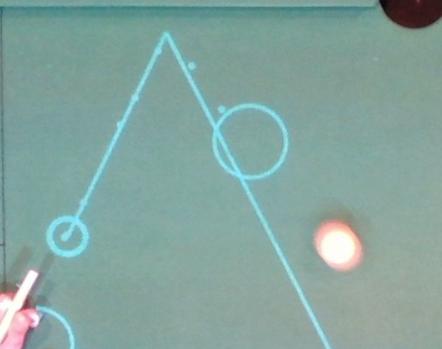
\includegraphics[width=1.0\linewidth]{../common/04_results/resources/simulation/rebound_angle_fast_pool/00_rail_rebound_angle_fast_pool_10.png}
        \caption{Ausfallswinkel bei starkem Stoss in Pool - 10}
        \label{fig:rebound_angle_fast_pool_10}
    \end{subfigure}
    \hfill
    \begin{subfigure}[b]{0.2\textwidth}
        \centering
        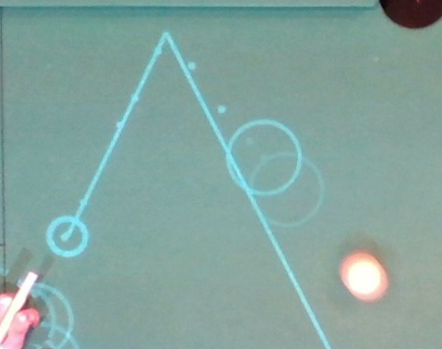
\includegraphics[width=1.0\linewidth]{../common/04_results/resources/simulation/rebound_angle_fast_pool/00_rail_rebound_angle_fast_pool_11.png}
        \caption{Ausfallswinkel bei starkem Stoss in Pool - 11}
        \label{fig:rebound_angle_fast_pool_11}
    \end{subfigure}
    \hfill
    \begin{subfigure}[b]{0.2\textwidth}
        \centering
        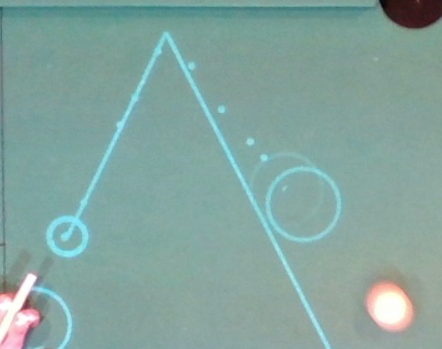
\includegraphics[width=1.0\linewidth]{../common/04_results/resources/simulation/rebound_angle_fast_pool/00_rail_rebound_angle_fast_pool_12.png}
        \caption{Ausfallswinkel bei starkem Stoss in Pool - 12}
        \label{fig:rebound_angle_fast_pool_12}
    \end{subfigure}
    \caption{Kugelverlauf nach Bandenkollision mit starkem Stoss - Pool}
    \label{fig:kugelverlauf_nach_bandenkollision_mit_starkem_stoss_pool}
\end{figure}

\newpage
Weiterhin werden anstelle der grösseren Pool-Kugeln kleinere Snooker-Kugeln verwendet. Dies kann ebenfalls einen
Einfluss auf das Zusammenspiel mit der Bande haben. Daher wurden dieselben Experimente, wie sie in diesem Kapitel vorgängig beschrieben
wurden, ebenfalls für Snooker-Kugeln durchgeführt, was den Abbildungen \ref{fig:kugelverlauf_nach_bandenkollision_mit_schwachem_stoss_snooker}
und \ref{fig:kugelverlauf_nach_bandenkollision_mit_starkem_stoss_snooker} zu entnehmen ist.
Das Verhalten ist im Wesentlichen dasselbe, der Ausfallswinkel ist in beiden Fällen viel zu gross.

\begin{figure}[h!]
    \centering
    \begin{subfigure}[b]{0.2\textwidth}
        \centering
        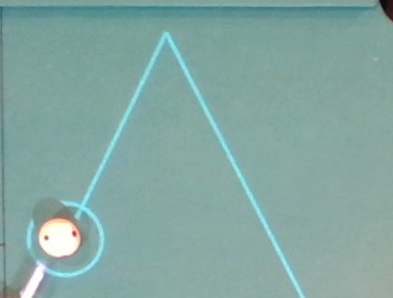
\includegraphics[width=1.0\linewidth]{../common/04_results/resources/simulation/rebound_angle_slow_snooker/00_rail_rebound_angle_slow_snooker_01.png}
        \caption{Ausfallswinkel bei schwachem Stoss in Snooker - 1}
        \label{fig:rebound_angle_slow_snooker_1}
    \end{subfigure}
    \hfill
    \begin{subfigure}[b]{0.2\textwidth}
        \centering
        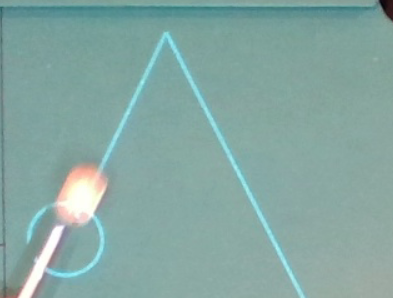
\includegraphics[width=1.0\linewidth]{../common/04_results/resources/simulation/rebound_angle_slow_snooker/00_rail_rebound_angle_slow_snooker_02.png}
        \caption{Ausfallswinkel bei schwachem Stoss in Snooker - 2}
        \label{fig:rebound_angle_slow_snooker_2}
    \end{subfigure}
    \hfill
    \begin{subfigure}[b]{0.2\textwidth}
        \centering
        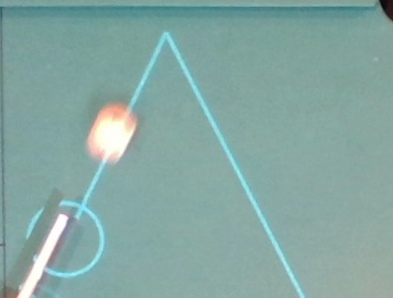
\includegraphics[width=1.0\linewidth]{../common/04_results/resources/simulation/rebound_angle_slow_snooker/00_rail_rebound_angle_slow_snooker_03.png}
        \caption{Ausfallswinkel bei schwachem Stoss in Snooker - 3}
        \label{fig:rebound_angle_slow_snooker_3}
    \end{subfigure}
    \hfill
    \begin{subfigure}[b]{0.2\textwidth}
        \centering
        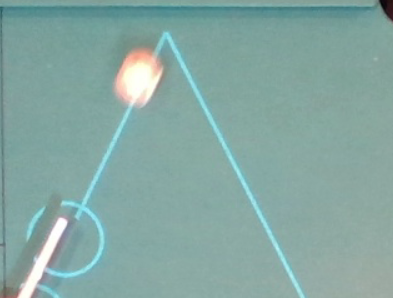
\includegraphics[width=1.0\linewidth]{../common/04_results/resources/simulation/rebound_angle_slow_snooker/00_rail_rebound_angle_slow_snooker_04.png}
        \caption{Ausfallswinkel bei schwachem Stoss in Snooker - 4}
        \label{fig:rebound_angle_slow_snooker_4}
    \end{subfigure}
    \hfill
    \begin{subfigure}[b]{0.2\textwidth}
        \centering
        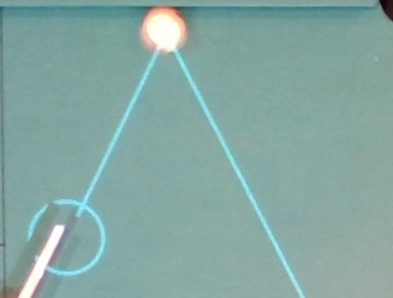
\includegraphics[width=1.0\linewidth]{../common/04_results/resources/simulation/rebound_angle_slow_snooker/00_rail_rebound_angle_slow_snooker_05.png}
        \caption{Ausfallswinkel bei schwachem Stoss in Snooker - 5}
        \label{fig:rebound_angle_slow_snooker_5}
    \end{subfigure}
    \hfill
    \begin{subfigure}[b]{0.2\textwidth}
        \centering
        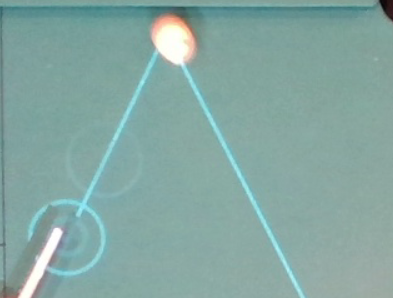
\includegraphics[width=1.0\linewidth]{../common/04_results/resources/simulation/rebound_angle_slow_snooker/00_rail_rebound_angle_slow_snooker_06.png}
        \caption{Ausfallswinkel bei schwachem Stoss in Snooker - 6}
        \label{fig:rebound_angle_slow_snooker_6}
    \end{subfigure}
    \hfill
    \begin{subfigure}[b]{0.2\textwidth}
        \centering
        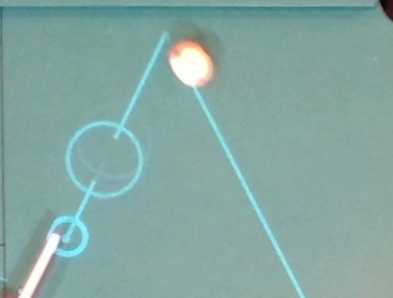
\includegraphics[width=1.0\linewidth]{../common/04_results/resources/simulation/rebound_angle_slow_snooker/00_rail_rebound_angle_slow_snooker_07.png}
        \caption{Ausfallswinkel bei schwachem Stoss in Snooker - 7}
        \label{fig:rebound_angle_slow_snooker_7}
    \end{subfigure}
    \hfill
    \begin{subfigure}[b]{0.2\textwidth}
        \centering
        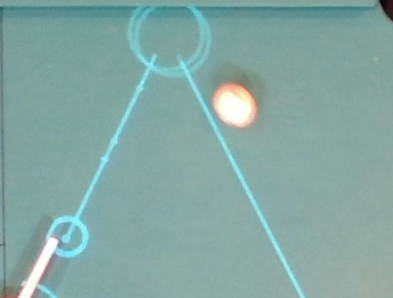
\includegraphics[width=1.0\linewidth]{../common/04_results/resources/simulation/rebound_angle_slow_snooker/00_rail_rebound_angle_slow_snooker_08.png}
        \caption{Ausfallswinkel bei schwachem Stoss in Snooker - 8}
        \label{fig:rebound_angle_slow_snooker_8}
    \end{subfigure}
    \hfill
    \begin{subfigure}[b]{0.2\textwidth}
        \centering
        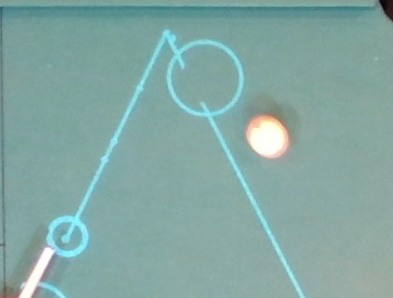
\includegraphics[width=1.0\linewidth]{../common/04_results/resources/simulation/rebound_angle_slow_snooker/00_rail_rebound_angle_slow_snooker_09.png}
        \caption{Ausfallswinkel bei schwachem Stoss in Snooker - 9}
        \label{fig:rebound_angle_slow_snooker_9}
    \end{subfigure}
    \hfill
    \begin{subfigure}[b]{0.2\textwidth}
        \centering
        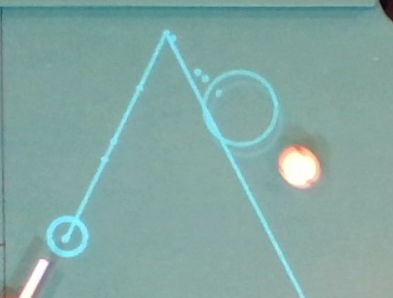
\includegraphics[width=1.0\linewidth]{../common/04_results/resources/simulation/rebound_angle_slow_snooker/00_rail_rebound_angle_slow_snooker_10.png}
        \caption{Ausfallswinkel bei schwachem Stoss in Snooker - 10}
        \label{fig:rebound_angle_slow_snooker_10}
    \end{subfigure}
    \hfill
    \begin{subfigure}[b]{0.2\textwidth}
        \centering
        \includegraphics[width=1.0\linewidth]{../common/04_results/resources/simulation/rebound_angle_slow_snooker/00_rail_rebound_angle_slow_snooker_11.png}
        \caption{Ausfallswinkel bei schwachem Stoss in Snooker - 11}
        \label{fig:rebound_angle_slow_snooker_11}
    \end{subfigure}
    \hfill
    \begin{subfigure}[b]{0.2\textwidth}
        \centering
        \includegraphics[width=1.0\linewidth]{../common/04_results/resources/simulation/rebound_angle_slow_snooker/00_rail_rebound_angle_slow_snooker_12.png}
        \caption{Ausfallswinkel bei schwachem Stoss in Snooker - 12}
        \label{fig:rebound_angle_slow_snooker_12}
    \end{subfigure}
    \caption{Kugelverlauf nach Bandenkollision mit schwachem Stoss - Snooker}
    \label{fig:kugelverlauf_nach_bandenkollision_mit_schwachem_stoss_snooker}
\end{figure}

\begin{figure}[h!]
    \centering
    \begin{subfigure}[b]{0.2\textwidth}
        \centering
        \includegraphics[width=1.0\linewidth]{../common/04_results/resources/simulation/rebound_angle_fast_snooker/00_rail_rebound_angle_fast_snooker_01.png}
        \caption{Ausfallswinkel bei starkem Stoss in Snooker - 1}
        \label{fig:rebound_angle_fast_snooker_1}
    \end{subfigure}
    \hfill
    \begin{subfigure}[b]{0.2\textwidth}
        \centering
        \includegraphics[width=1.0\linewidth]{../common/04_results/resources/simulation/rebound_angle_fast_snooker/00_rail_rebound_angle_fast_snooker_02.png}
        \caption{Ausfallswinkel bei starkem Stoss in Snooker - 2}
        \label{fig:rebound_angle_fast_snooker_2}
    \end{subfigure}
    \hfill
    \begin{subfigure}[b]{0.2\textwidth}
        \centering
        \includegraphics[width=1.0\linewidth]{../common/04_results/resources/simulation/rebound_angle_fast_snooker/00_rail_rebound_angle_fast_snooker_03.png}
        \caption{Ausfallswinkel bei starkem Stoss in Snooker - 3}
        \label{fig:rebound_angle_fast_snooker_3}
    \end{subfigure}
    \hfill
    \begin{subfigure}[b]{0.2\textwidth}
        \centering
        \includegraphics[width=1.0\linewidth]{../common/04_results/resources/simulation/rebound_angle_fast_snooker/00_rail_rebound_angle_fast_snooker_04.png}
        \caption{Ausfallswinkel bei starkem Stoss in Snooker - 4}
        \label{fig:rebound_angle_fast_snooker_4}
    \end{subfigure}
    \hfill
    \begin{subfigure}[b]{0.2\textwidth}
        \centering
        \includegraphics[width=1.0\linewidth]{../common/04_results/resources/simulation/rebound_angle_fast_snooker/00_rail_rebound_angle_fast_snooker_05.png}
        \caption{Ausfallswinkel bei starkem Stoss in Snooker - 5}
        \label{fig:rebound_angle_fast_snooker_5}
    \end{subfigure}
    \hfill
    \begin{subfigure}[b]{0.2\textwidth}
        \centering
        \includegraphics[width=1.0\linewidth]{../common/04_results/resources/simulation/rebound_angle_fast_snooker/00_rail_rebound_angle_fast_snooker_06.png}
        \caption{Ausfallswinkel bei starkem Stoss in Snooker - 6}
        \label{fig:rebound_angle_fast_snooker_6}
    \end{subfigure}
    \hfill
    \begin{subfigure}[b]{0.2\textwidth}
        \centering
        \includegraphics[width=1.0\linewidth]{../common/04_results/resources/simulation/rebound_angle_fast_snooker/00_rail_rebound_angle_fast_snooker_07.png}
        \caption{Ausfallswinkel bei starkem Stoss in Snooker - 7}
        \label{fig:rebound_angle_fast_snooker_7}
    \end{subfigure}
    \hfill
    \begin{subfigure}[b]{0.2\textwidth}
        \centering
        \includegraphics[width=1.0\linewidth]{../common/04_results/resources/simulation/rebound_angle_fast_snooker/00_rail_rebound_angle_fast_snooker_08.png}
        \caption{Ausfallswinkel bei starkem Stoss in Snooker - 8}
        \label{fig:rebound_angle_fast_snooker_8}
    \end{subfigure}
    \hfill
    \begin{subfigure}[b]{0.2\textwidth}
        \centering
        \includegraphics[width=1.0\linewidth]{../common/04_results/resources/simulation/rebound_angle_fast_snooker/00_rail_rebound_angle_fast_snooker_09.png}
        \caption{Ausfallswinkel bei starkem Stoss in Snooker - 9}
        \label{fig:rebound_angle_fast_snooker_9}
    \end{subfigure}
    \hfill
    \begin{subfigure}[b]{0.2\textwidth}
        \centering
        \includegraphics[width=1.0\linewidth]{../common/04_results/resources/simulation/rebound_angle_fast_snooker/00_rail_rebound_angle_fast_snooker_10.png}
        \caption{Ausfallswinkel bei starkem Stoss in Snooker - 10}
        \label{fig:rebound_angle_fast_snooker_10}
    \end{subfigure}
    \hfill
    \begin{subfigure}[b]{0.2\textwidth}
        \centering
        \includegraphics[width=1.0\linewidth]{../common/04_results/resources/simulation/rebound_angle_fast_snooker/00_rail_rebound_angle_fast_snooker_11.png}
        \caption{Ausfallswinkel bei starkem Stoss in Snooker - 11}
        \label{fig:rebound_angle_fast_snooker_11}
    \end{subfigure}
    \hfill
    \begin{subfigure}[b]{0.2\textwidth}
        \centering
        \includegraphics[width=1.0\linewidth]{../common/04_results/resources/simulation/rebound_angle_fast_snooker/00_rail_rebound_angle_fast_snooker_12.png}
        \caption{Ausfallswinkel bei starkem Stoss in Snooker - 12}
        \label{fig:rebound_angle_fast_snooker_12}
    \end{subfigure}
    \caption{Kugelverlauf nach Bandenkollision mit starkem Stoss - Snooker}
    \label{fig:kugelverlauf_nach_bandenkollision_mit_starkem_stoss_snooker}
\end{figure}

\newpage
An dieser Stelle kann festgehalten werden, dass die Bande des Billardtisches nicht die erwarteten Eigenschaften
aufweist, was wahrscheinlich daran liegt, dass es ein sehr günstig erhältliches Produkt und dementsprechend auch
die Qualität ist. Anzumerken ist, dass während dem Spielen aufgefallen ist, dass das rechte Bandensegment die
Eigenschaften besser erfüllt. Festgehalten wird auch die Tatsache, dass das Verwenden der Snooker-Kugeln einen
Einfluss haben kann, dieser aber nicht so stark ins Gewicht fällt wie das grundlegende Fehlverhalten
der Bande.

Dass die Banden nicht in Ordnung sind, zeigt ein weiterer durchgeführter Test. Demnach muss eine Kugel insgesamt vier Mal über
die Tischlänge oder fünf Mal über die Tischbreite laufen, wenn sie stark angespielt wird\cite{sport64:bandengummi}.
Auf dem verwendeten Tisch schafft die Kugel nur deren 2.5, respektive 3 Läufe.

\newpage
\subsubsection{Diskussion}
Nach dem Autor des Buches \glqq The illustrated principles of pool and billiards\grqq{} gibt es diverse Einflüsse,
die den Ausfallswinkel der Kugel nach einer Bandenkollision beeinträchtigen. Laut ihm ist daher eine mittlere
Geschwindigkeit zu bevorzugen, welche diese unerwünschten Effekte minimal hält\cite{book:the_ilustrated_principles_of_pool_and_billiards}.
Leider findet sich keine Aussage, wie stark ein schwacher, mittlerer oder starker Stoss genau ist.

Demgegenüber steht die Aussage der Autoren des Papers \glqq A theoretical analysis of billiard ball dynamics under cushion impacts\grqq, welche ebenfalls
gewisse Abweichungen festgestellt haben, jedoch im Schnitt durchaus einen linearen Zusammenhang feststellen konnten.

Einen Einfluss auf diese Untersuchungen hat die verwendete Hardware, namentlich der Billardtisch und die
zugehörigen Kugeln. So ist das Verhalten einer Kugel nach einer Bandenkollision vor allem vom verwendeten Gummi der
Bande abhängig. Dadurch kann es zu gewichtigen Unterschieden kommen.
Diese theoretischen und praktischen Erkenntnisse bilden dennoch die Grundlage in der vorliegenden Arbeit,
da davon ausgegangen werden kann, dass im professionellen  Umfeld ein Billardtisch diese genannten Eigenschaften aufweisen muss.

Leider gilt dies nicht für den in dieser Arbeit verwendeten Billardtisch.
Dessen Bandeneigenschaften entsprechen keinesfalls den Vorgaben und ist für den professionellen und privaten Gebrauch ungeeignet,
da wahrscheinlich ein günstiges Gummi verwendet wurde.
Ein entsprechendes Statement ist auch aus einer Bewertung aus dem Onlineshop zu entnehmen, siehe Abbildung \ref{fig:bewertung_billardtisch}.

\begin{figure}[h!]
    \begin{center}
        \includegraphics[width=0.3\linewidth]{../common/04_results/resources/simulation/00_bewertung_billardtisch.png}
    \end{center}
    \caption{Bewertung zu Billardtisch\cite{gonser:billardtisch}}
    \label{fig:bewertung_billardtisch}
\end{figure}

Demnach wird festgehalten, dass die in dieser Arbeit verwendete Theorie durchaus funktioniert und der Realität
standhält, im Zusammenhang mit dem verwendeten Billardtisch dennoch leider nicht verwendbar ist aufgrund der schlechten
Qualität desselbigen.
% TODO: vergleich ausschnitte vom video und simulation zu bestimmten Ereigniszeitpunkten für Diskussion über Weg der weissen Kugel
